\chapter{Szerveroldali folyamatok implementációi}

A megjelenítési réteg alatt található szerveroldali folyamatok implementációja során a~kiszolgáló infrastruktúra kialakítására, a Node.js-alkalmazás fejlesztésére, a konténerizált környezet kialakítására, valamint a videófeldolgozásra fókuszálunk ebben a fejezetben.

\section{A virtuális privát felhő komponensei}\label{sec:vpc}

A szerveroldal erőforrásait igyekeztem mindet egy közös VPC-be szervezni, amely lehetővé teszi, hogy a komponensek egymást lássák, és biztonságosan kommunikáljanak egymással alhálózataik között. A VPC-n belül az összetartozó elemekhez két-két alhálózatot hoztam létre. A legtöbb AWS-szolgáltatás a magas rendelkezésreállás érdekében legalább kettő konkrét adatközpontba kell kitelepítése kerüljön, azaz az AWS saját terminológiáját használva: két \emph{Availibility Zone}-ba (AZ) kell elhelyezésre kerüljenek a konkrét erőforrások. Ennek megfelelően az eu-central-1 régió alatti \emph{eu-central-1a} és \emph{eu-central-1b} AZ-ba szerveztem az egyes alhálózataim. Az alhálózatok közötti forgalom irányítását útválasztó táblák (angolul \emph{route table}) segítségével végeztem, amelyek biztosítják, hogy a komponensek közötti kommunikáció megfelelően működjön. Az útválasztó táblák konkrét bejegyzéseit, valamint a felhasznált IP-tartományokat is tartalmazza \az+\refstruc{fig:vpc}.

\begin{figure}
  \centering
  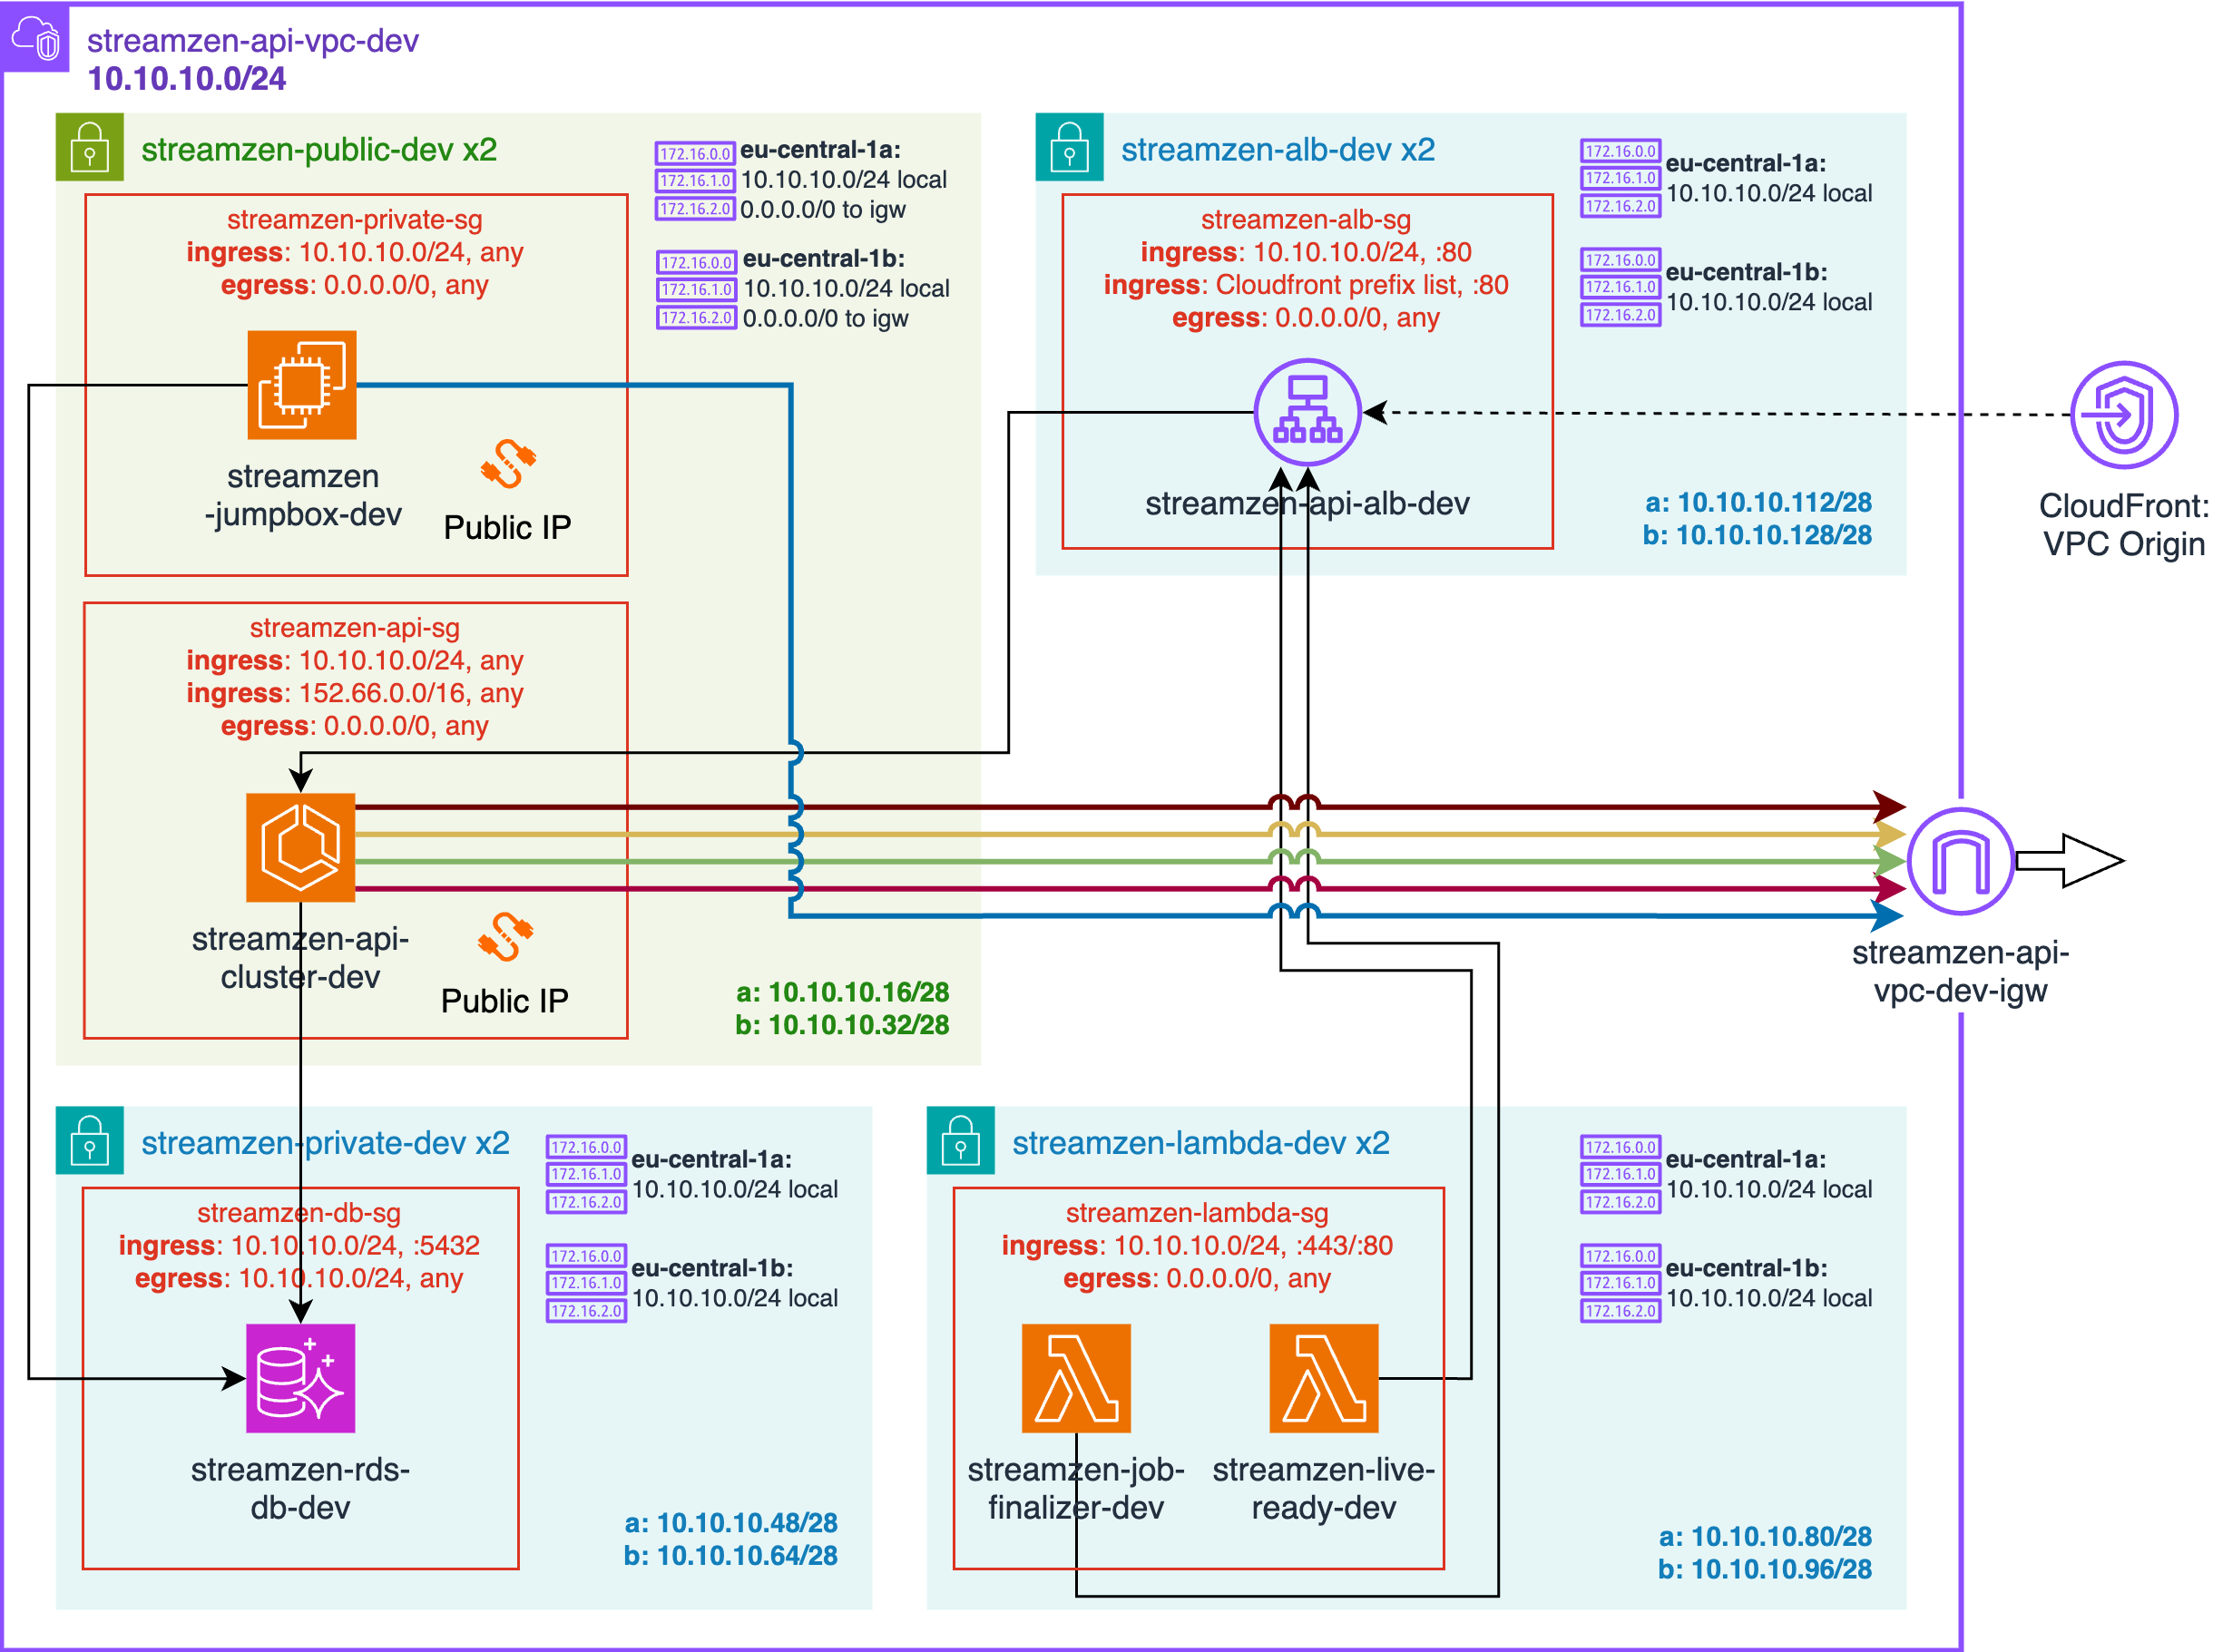
\includegraphics[width=150mm, keepaspectratio]{figures/dipterv_vpc.png}
  \caption{Részletes architektúraábra a VPC-ről.}
  \label{fig:vpc}
\end{figure}

Az ábráról leolvashatóak még a Security Groupok, azaz virtuális állapotmentes tűzfalak, ezek a komponensek vörös keretként látszódnak az ábrán és \verb|-sg| végződésűek neveik. Ezek a tűzfalak úgy kerültek kialakításra, hogy a csupán a ténylegesen szükséges IP-tartományokat és portokat engedélyezzék a kommunikációhoz.

A legelső belépési pontja egy kérésnek az ALB-példány, amely privát alhálózatra lett bekötve. Privátnak minősül egy alhálózat, amennyiben nincs közvetlen internetkapcsolata, nem kerül bekötésre az útválasztó táblájába IGW.

Habár bevezetésre került egy Internet Gateway (IGW), fontos megjegyezni, hogy nem azért, hogy a kliensoldali erőforrás -- a CloudFront-disztribúció -- elérhesse a szerveroldalt, hiszen azt megvalósítja egy VPC Originen keresztül, amely működési lényege, hogy számára nem szükségeltetik bevezetni publikus alhálózatot, a disztribúció közvetlen összeköttetést tud összehozni VPC-n belül elrejtett hálózati erőforrásokkal, azaz a mi ALB-példányunkkal is. Az IGW bevezetésének indokait a következő bekezdések tisztázzák.

Az ECS-klaszter, amely a Node.js-alkalmazást futtatja és összeköttetésre kerül az~ALB-vel, viszont már publikus alhálózatban helyezkedik el. A Security Groupja úgy lett beállítva, hogy a VPC-n belüli eszközöket engedje be, illetve azt az IP-tartományt, amelyben az AuthSCH is fut (ez a Schönherz Kollégium hálózati tartománya, a 152.66.0.0/16).

A szervernek fontos a kapcsolódása az adatbázisra, amely egy külön privát alhálózatot kapott, abba a Security Group csupán a PostgreSQL-re jellemző 5432 porton keresztül enged és csak a VPC-belülről forgalmat, hasonlóképp kifelé is csak a VPC-n belülre enged.

Az ECS-klaszterben működő szervernek több a privát hálózaton kívül működő szolgáltatás felé kell tudnia kommunikálni. Ezek a VPC-n kívüli komponensek \az+\refstruc{fig:nonvpc} segítségével kerülnek vizuálisan ismertetésre.

\begin{figure}
  \centering
  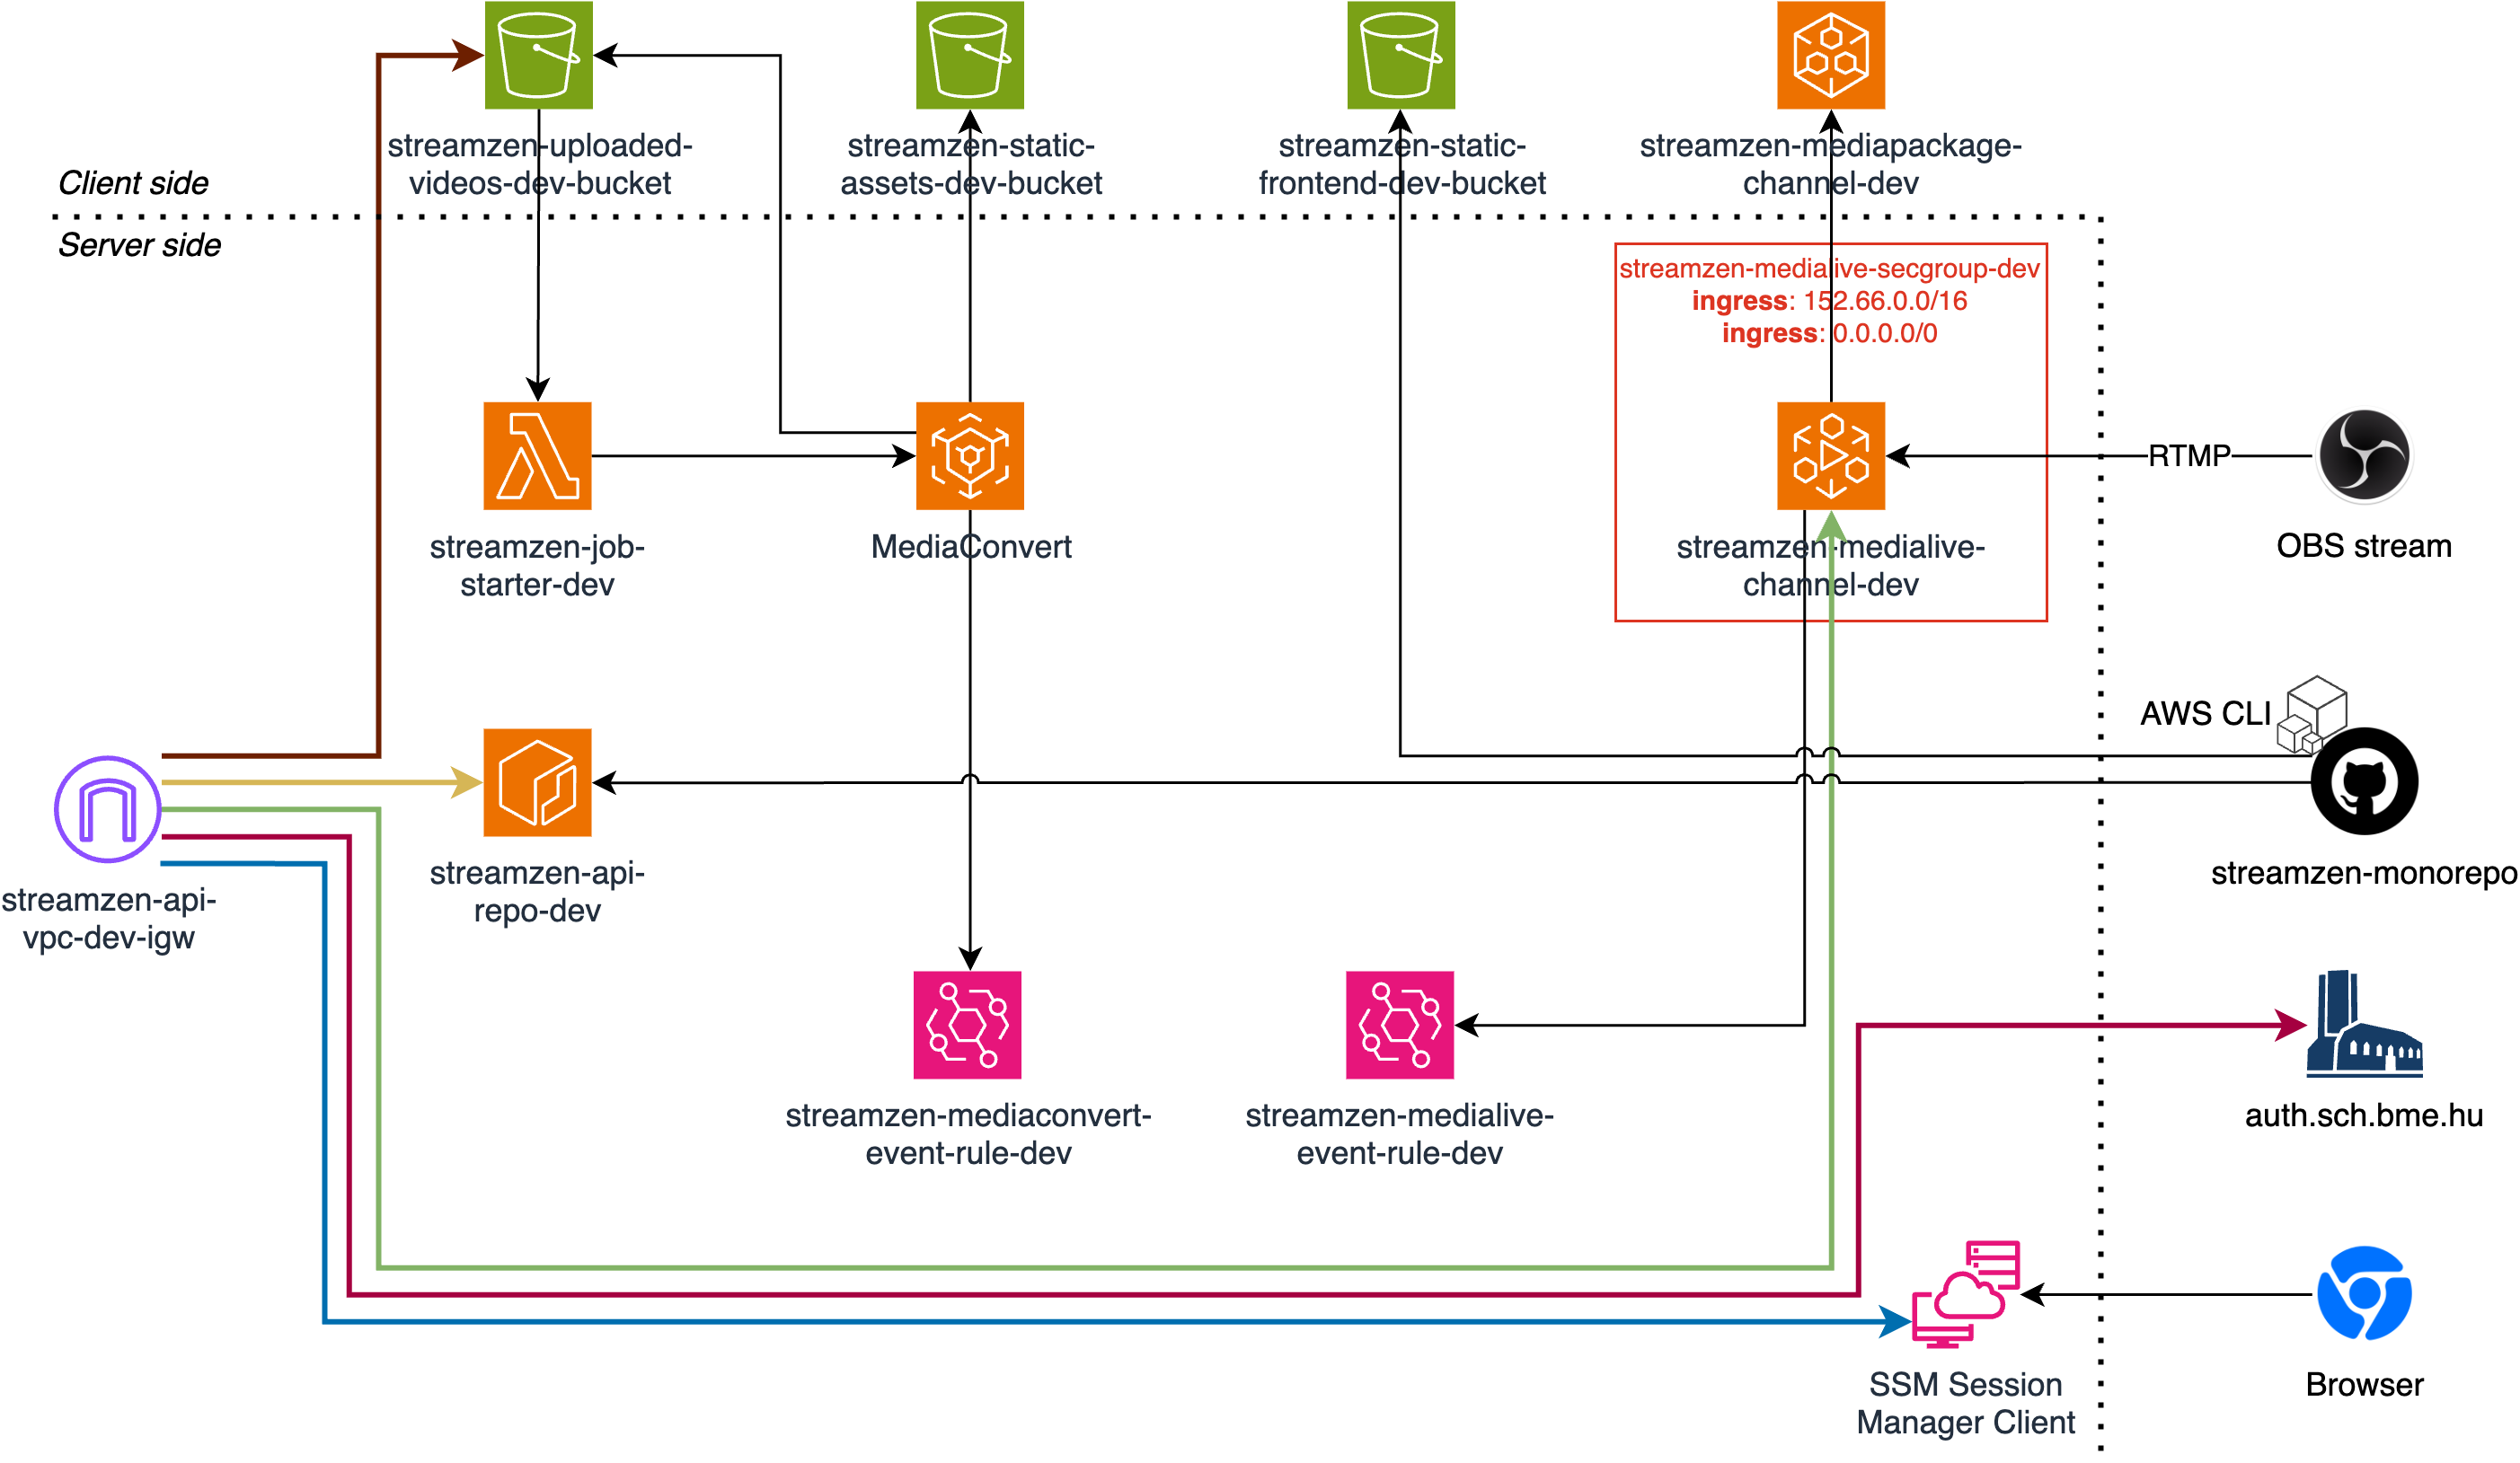
\includegraphics[width=150mm, keepaspectratio]{figures/dipterv_nonvpc.png}
  \caption{Részletes architektúraábra a VPC-ből kifelé és befelé kommunikáló komponensekkel.}
  \label{fig:nonvpc}
\end{figure}

\Az+\refstruc{fig:nonvpc} ábra és \az+\refstruc{fig:vpc} együttesen mutatja be az Internet Gateway-en keresztüli kommunikációs útvonalakat, azonos színű vonalak egyazon kommunikációs útvonalat jelölik. Ennek megfelelően az előző bekezdésben jelölt AuthSCH-t elérő kommunikációs útvonalat követi le a piros vonal. A sárga vonal jelöli azt, ahogy az ECS-klaszter eléri az~ECR`|tárolót a Docker-kép letöltésére. A zöld vonal jelöli a szerver és a MediaLive`|csatorna közti utat, amelyen keresztül a szerver elindítja az vételt a csatornán. Végül pedig a barna vonal jelöli a videófeltöltés folyamatát az S3-vödörbe a szerveren keresztül.

Léteznek különféle hálózati erőforrástípusok, hogy privát alhálózatban helyezzünk el egy ECS-ben futó szervert, illetve akár Lambda-függvényeket, amelyek kommunikálnak VPC-n kívüli eszközökkel. Ilyen erőforrástípus a \emph{NAT Gateway}, amely Network Address Translation (NAT) szolgáltatás, és amennyiben adunk neki egy állandó publikus IP-címet (Amazon Elastic IP szolgáltatással), úgy képes azon keresztül az internet felé forgalmazást biztosítani a VPC erőforrásai számára, kinti erőforrásoknak viszont befelé már nem. Ez megoldotta volna az AuthSCH felé kommunikálást. Egy másik lehetőség lett volna a~\emph{VPC Endpointok} alkalmazása, amelyek interfészt szolgáltatnak bizonyos AWS-en belüli szolgáltatások felé anélkül, hogy az elhagyná az adatközpontot. A bizonyos szolgáltatások közé tartozik a CloudWatch Logs, az ECR, az ECS-hez tartozó egyéb szolgáltatások, az EventBridge és az S3 is. Ezt a biztonsági kockázatot a kísérletem szempontjából nem kívántam megelőzni, az igazán szükséges védelmi réteget a Security Group is megvalósítja, a privát alhálózat csupán plusz egy réteget jelent nagy kockázatú, vegyes forgalmat kezelő vállalati rendszerek kivitelezése során, az én esetemben a költségek és a bonyolultság erősen megnőtt volna jelölt erőforrások bekötésével.

A hálózat építése tégláról téglára került kivitelezésre, a fejlesztési/tervezési fázisban ezért érdemesnek tartottam a tesztelés során \emph{``jumpbox''} jelleggel bevezetni egy EC2`|példányt, amely a publikus alhálózatban helyezkedik el. Viszont az elérése nem kívántam jelszavakat, SSH-kulcsokat kezelni, ezért az AWS Systems Manager (SSM) Session Manager szolgáltatását használtam, amely lehetővé tette, hogy a webes konzolon keresztül SSH-kapcsolatot létesítsek az EC2-példánnyal anélkül, hogy közvetlenül elérné azt. Az~EC2-es példány létrehozása után egy ágenset kellett volna telepítsek, amely erre felkészíti magát a virtuális gépet, azonban ezt a telepítési folyamatot is automatizáltam a Systems Manager Host Management szolgáltatásával, amely lehetővé teszi az EC2-példányok központi kezelését. A jumpbox segítségével tudtam pingelgetni a hálózati eszközök interfészeit, illetve a~Security Groupok beállításait is tesztelni, és akár az RDS-adatbázison is futtatni egyszerű lekéréseket, sémamigrációkat.

\section{A Node.js-alkalmazás fejlesztése}\label{sec:nodejs}

A NestJS keretrendszerben írt Node.js-alkalmazások modulokra bomlanak, az egyes modulok \emph{controller} rétegre és \emph{service} rétegre válnak ketté, a javaslat, hogy az előbbi réteg osztályaiban a forgalomirányítást valósítsuk meg, a későbbiben pedig a konkrét szolgáltatásszintű üzleti logikát, a számításokat, adattisztítást, adatelérést valósítsuk meg. A~modulok implementációjában az egyes \emph{service} és \emph{controller} típusú osztályok példányainak beinjektálását, illetve azok életciklusáról való gondoskodást a NestJS által biztosított Dependency Injection (DI) rendszer valósítja meg.

Az elkészült webszerver-alkalmazás egy REST API-t valósít meg. A benne kialakításra került modulok a következő funkciókat látják el:

\begin{enumerate}
  \item \verb|AuthModule|: A felhasználók azonosításáért és jogosultságkezeléséért felelős modul.
  \item \verb|PrismaModule|: Csupán behúzza a rendszerbe a projektbe telepített Prisma ORM-et mint service.
  \item \verb|UsersModule|: A felhasználók kezeléséért felelős modul, amely a felhasználók CRUD-műveleteit valósítja meg.
  \item \verb|VideoModule|: A videók kezeléséért felelős modul, amely a videók feltöltését és metaadatainak kezelését valósítja meg.
\end{enumerate}

\subsection{Az adatbázisséma}

\Az+\refstruc{fig:prismaliser} mutatja be a Prisma-ban írt Prisma-sémát. A séma tartalmaz jövőbeli felhasználásra szánt elemeket, az egyszerűségre törekszik a séma, csupán a lényeges adatokat tároljuk le.

A \verb|User| entitás reprezentálja a felhasználókat, akik megfelelő \verb|role| attribútumérték esetén feltölteni tudnak a weboldalra. A \verb|role| attribútum típusát enum típusra állítottam, amelynek értékei a \verb|USER| és \verb|ADMIN|. A \verb|User|-nek számított attribútuma a \verb|vods| és a~\verb|crewMemberships|.

A \verb|Vod| entitás a feltöltött videók metaadatait reprezentálja. A \verb|Vod| entitásnak meg kell adni létrehozáskor egy \verb|User| kapcsolatot, amely a feltöltő felhasználót reprezentálja. Ezenkívül fontos attribútuma a \verb|state|, amely a videó állapotát reprezentálja. A \verb|state| attribútum enum típusú, lehet értéke \verb|UNPROCESSED| (ez a létrehozáskori érték), lehet \verb|UPLOADED| (amikor feltöltésre került), \verb|PROCESSING| (amikor már a MediaConvert dolgozik az átalakításán), \verb|PROCESSED| (amikor véget ért a MediaConvert-job), vagy pedig \verb|FAILED| (amennyiben hiba történt valamelyik fázisban). Segít a videó állapotának nyomon követésében a~\verb|statePercent| attribútum is, amely a MediaConvert által visszaadott százalékos értéket tárolja le.

A \verb|CrewMembership| entitáshoz tartozó tábla a \verb|Vod| és a \verb|User| entitások közötti illesztő tábla (angolul \emph{join table}), saját attribútumokat tud ehhez a kapcsolathoz hozzáadni, kardinalitás szempontjából egy \verb|CrewMembershipnek| csak egy \verb|User|-t és csak egy \verb|Vod|-ot kell kötnie. Egy \verb|Vod|-nak persze több \verb|CrewMembership|-je is lehet, ugyanígy \verb|User|-nek is. Ez az entitás és a \verb|ViewCounter| -- amely a megtekintések számlálóját lett volna hivatott reprezentálni -- aktívan nem került felhasználásra a fejlesztés során, tervezésben maradt csupán, nem volt esszenciális a végső cél megvalósításához.

\begin{figure}[h]
  \centering
  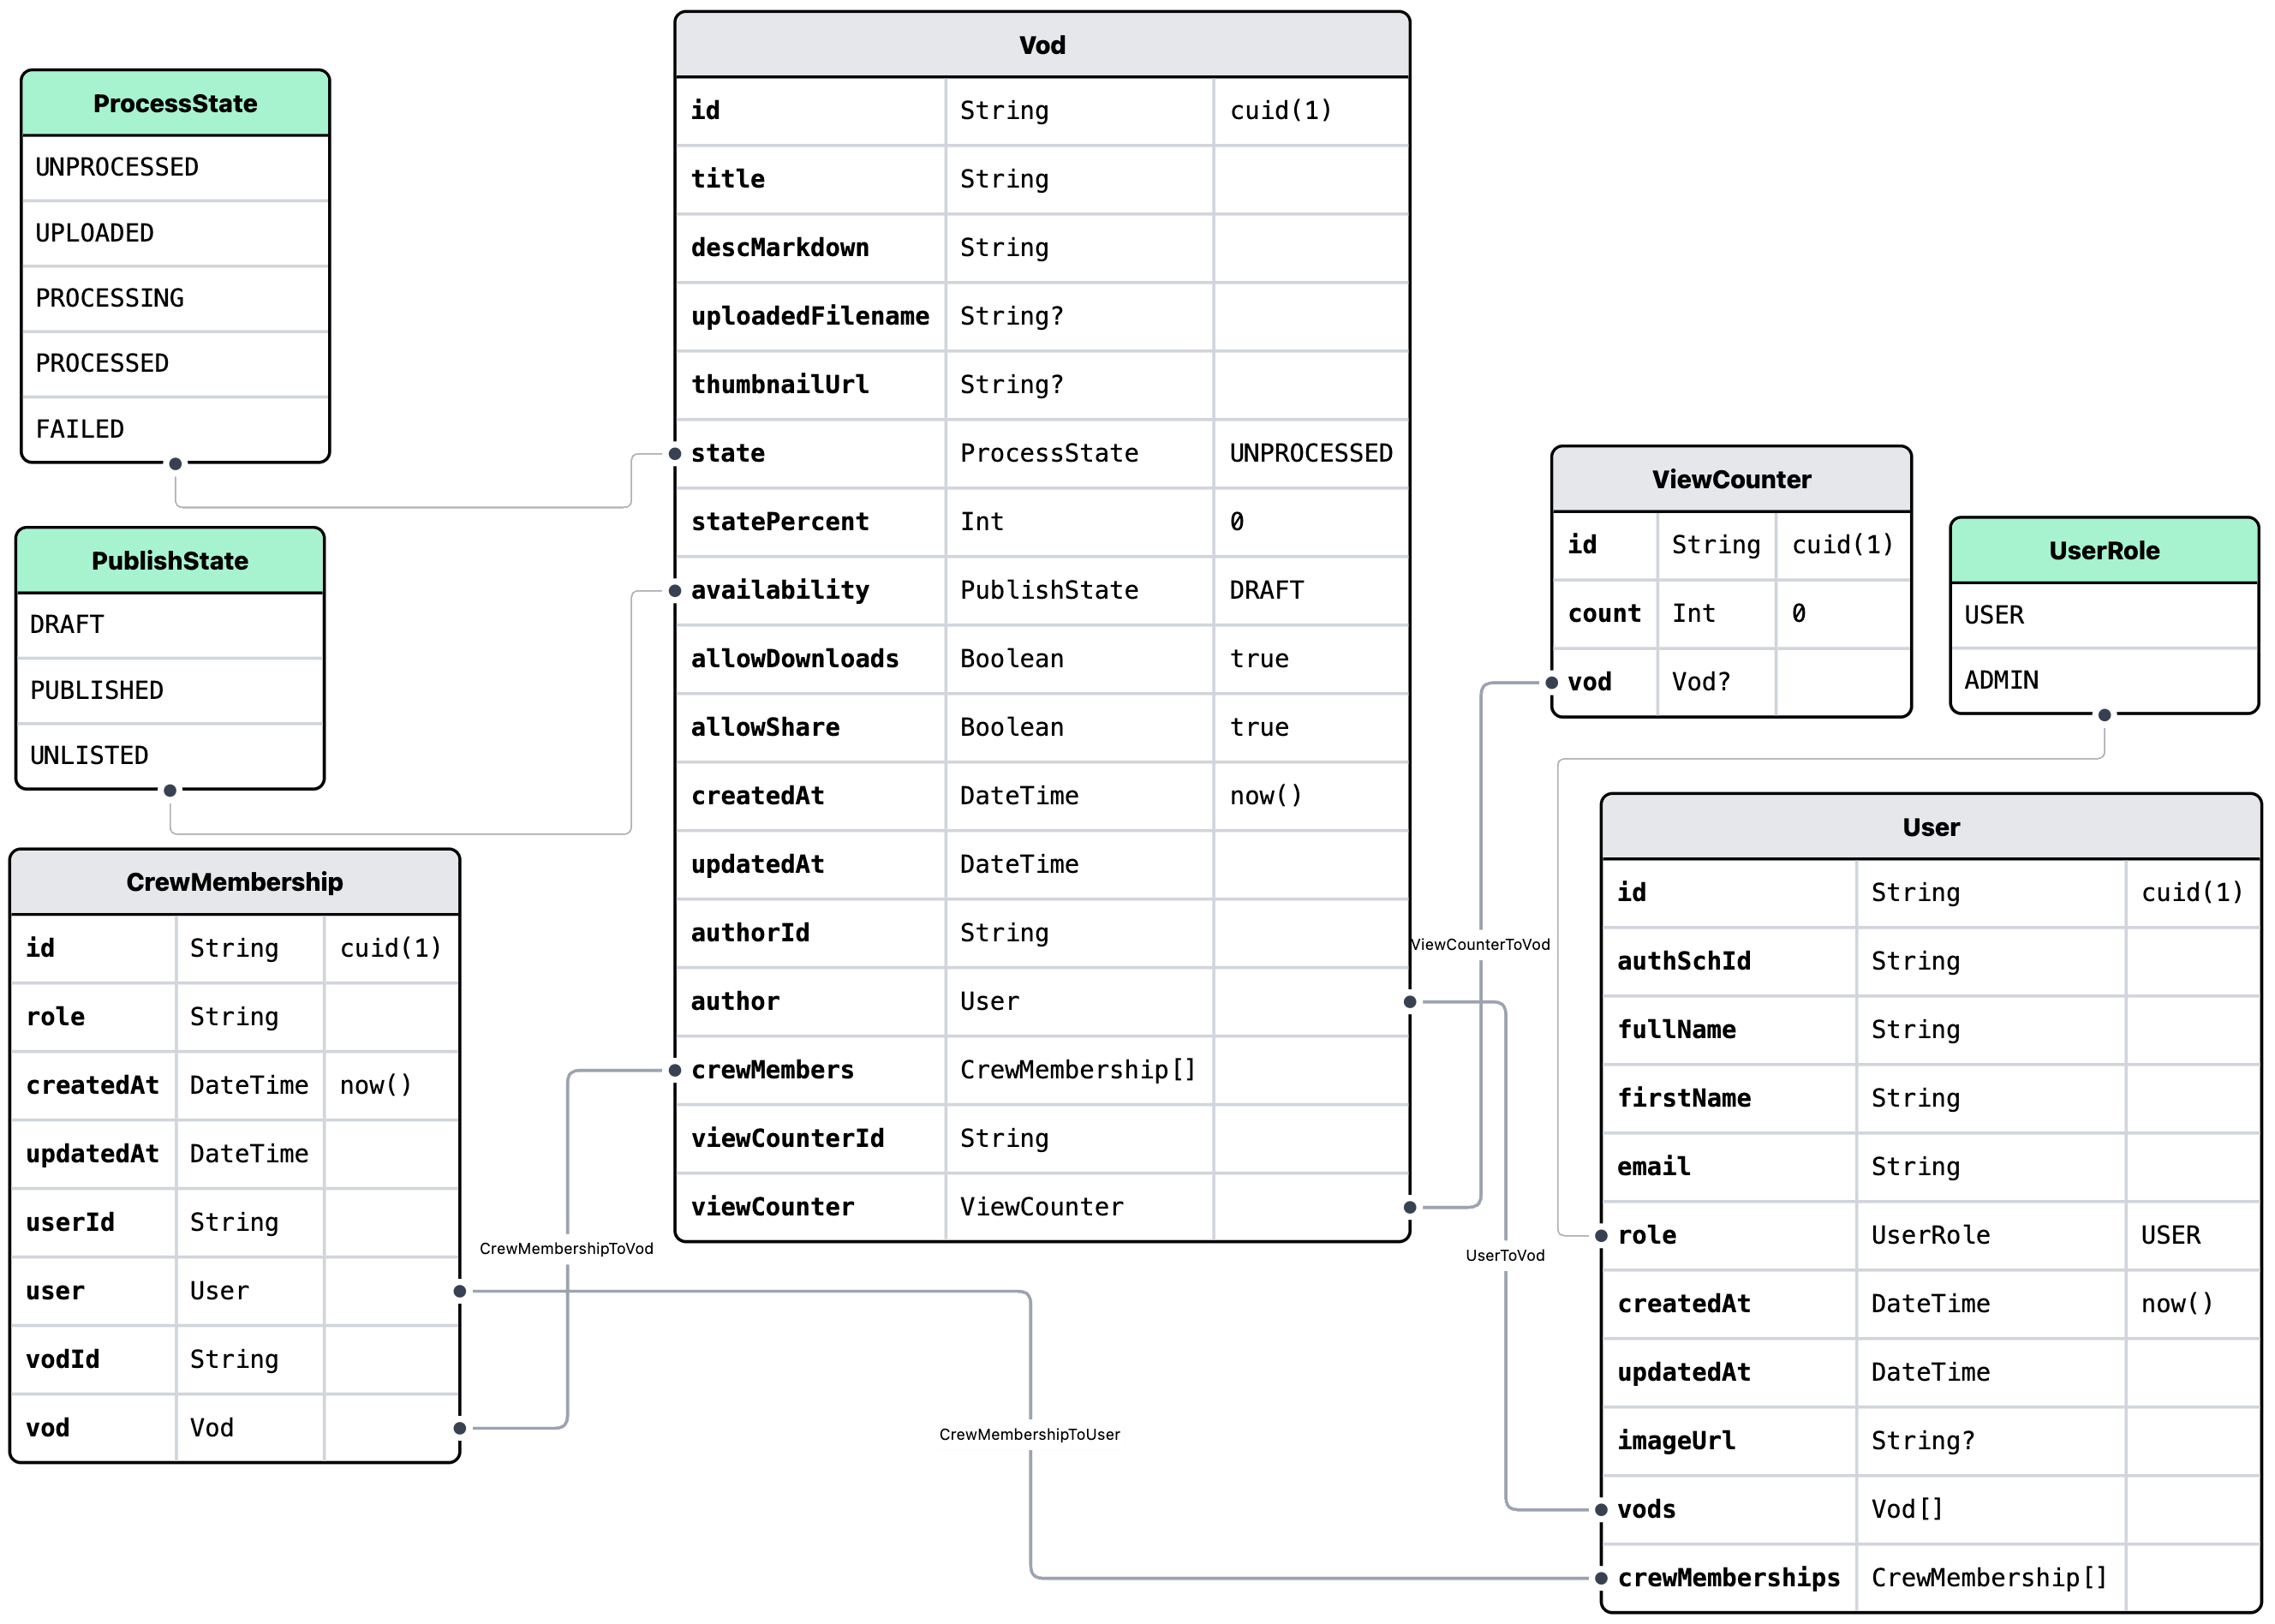
\includegraphics[width=150mm, keepaspectratio]{figures/prismaliser.png}
  \caption{A Prisma-séma vizuális reprezentációja.}
  \label{fig:prismaliser}
\end{figure}

\subsection{Környezeti változók}\label{sec:envvars}

Az alkalmazásnak korábbi alfejezetekben már kiderült, hogy vannak külső függőségei. Ezen függőségekhez való hozzáféréshez a környezeti változók használata elengedhetetlen. A ECS-ben futó konténer környezeti változóinak beállítására az ECS is ad lehetőséget \az+\ref{lst:mainApi}. kódrészlet mutatja be a Terraform-kód egy részletét, amely átpasszolja az alkalmazás számára a következő fontos paramétereket.

Az AuthSCH SSO-ban felvett OAuth-kliensünk\cite{ietf-oauth-security-topics-13} azonosítóját és titkos kulcsát a~\verb|AUTHSCH_CLIENT_ID| és \verb|AUTHSCH_CLIENT_SECRET| környezeti változók tárolják, ezek értékeit ahogy a kódból is látható egy-egy SSM Parameter Store-ból szerzi meg a CI/CD`|folyamat futtatása során a Terraform-kliensünk (értsd: a referált erőforrás elején \verb|data| kulcsszó jelöli, hogy \emph{data source}-ként éri kéri le a Terraform az AWS CDK-n keresztül az értékét). Ezen Param Store kulcs-érték párokhoz az értéket az AuthSCH saját oldalán szereztem meg \url{auth.sch.bme.hu} oldalon található webes felületén, ahol korábban már megszerzett SCHAcc-fiókomba való belépés után új OAuth-kliens beregisztrálása után tudtam magamnak generálni a kívánt értékeket (ID és client secret).

Egy felhasználónevet és jelszót (\verb|POSTGRES_USER| és \verb|POSTGRES_PASSWORD|) is meg kell tudjuk adni környezeti változón keresztül az alkalmazásunknak, amellyel autentikál az~adatbázisba, ezek értékét is SSM Param Store-okba tettem bele, viszont a felhasználónevet már magam találtam ki, a jelszót pedig magam generáltam kézzel.

Az alkalmazásnak tudnia kell bizonyos átirányítások lekezelésére a kliensünk bázis URL-jét, így azt megadtam környezeti változóban (\verb|FRONTEND_CALLBACK|). A doménnevet változtathatónak véltem hagyni, ezért is került Terraform-változóba az értéke (\verb|var.domain_name|).

Ezenkívül még szükség van egy titkos kulcsra, amely a JWT-tokenek aláírására szolgál (\verb|JWT_SECRET|), ezt is SSM Param Store-ból szerzi be az alkalmazásunk, illetve ezt is már én töltöttem be, miután kézzel generáltam egyet.

A feltöltött videókat tároló S3-vödör nevét (\verb|AWS_S3_UPLOADED_BUCKET|) az általam kitalált nevezéktani konvenciók alapján töltöm be, illetve az S3-vödör régióját (\verb|AWS_S3_REGION|) pedig természetesen arra a régióra állítom, ahová az erőforrások főképp telepítésre kerültek (és ahova az S3-vödör is került).

\begin{minipage}{0.92\textwidth}
  \begin{lstlisting}[
    caption=Az ECS-taszk környezeti változóinak feltöltése Terraformban.,
    label=lst:mainApi,
    style=tf,
    basicstyle=\fontsize{10}{12}\ttfamily,
  ]
task_environment = {
  AUTHSCH_CLIENT_ID = data.aws_ssm_parameter.these["authsch-client-id"].value
  AUTHSCH_CLIENT_SECRET = data.aws_ssm_parameter.these["authsch-client-secret"].value
  POSTGRES_USER = data.aws_ssm_parameter.these["db-username"].value
  POSTGRES_PASSWORD = data.aws_ssm_parameter.these["db-password"].value
  FRONTEND_CALLBACK = "https://${var.domain_name}"
  JWT_SECRET = data.aws_ssm_parameter.these["api-jwt-secret"].value
  AWS_S3_REGION = var.region
  AWS_S3_UPLOADED_BUCKET = "streamzen-uploaded-videos-${var.environment}-bucket"
}
\end{lstlisting}
\end{minipage}

\section{A konténerizált környezet}

A konténerizált webalkalmazás kialakítására a Docker ökoszisztémájának eszközeit vettem alkalmazásba. A fejlesztés során a \emph{Docker Desktop} alkalmazást használtam, amely lehetővé tette a konténerek helyi futtatását, a \emph{Docker Compose} segítségével pedig a~Node.js-alkalmazás mellé felvettem egy PostgreSQL-adatbázis konténerét is, azok között a Compose-kóddal a konténerek közötti kommunikációt is könnyen meg tudtam valósítani.

\begin{figure}[h]
  \centering
  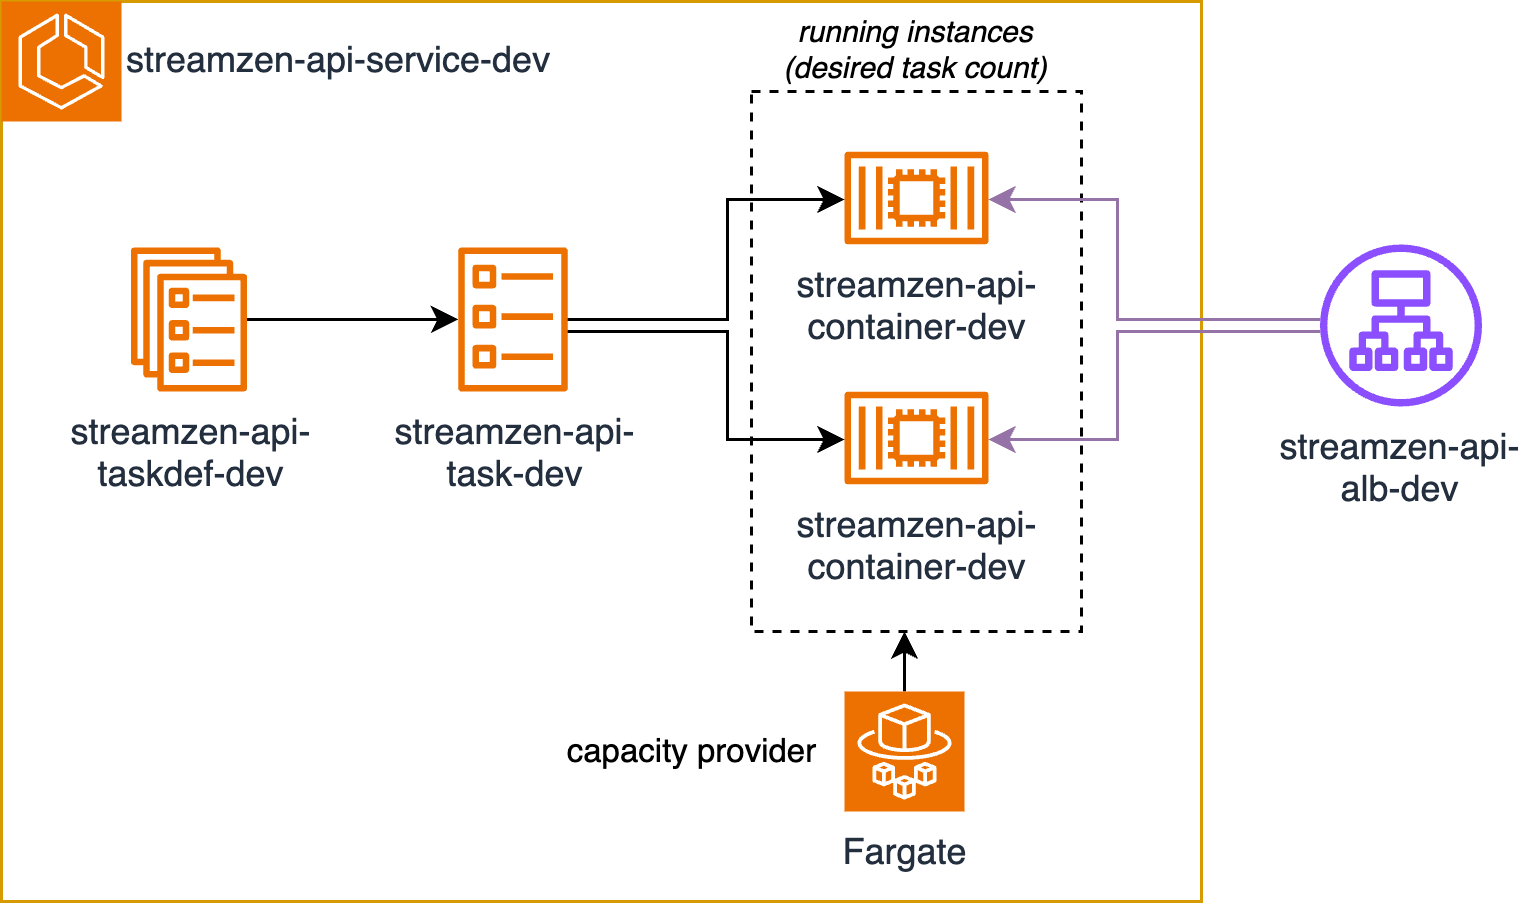
\includegraphics[width=100mm, keepaspectratio]{figures/dipterv_ecs.png}
  \caption{Az ECS-klaszter elemei.}
  \label{fig:ecscluster}
\end{figure}

Az élesítése a Node.js-alkalmazásnak a korábban is ismertetett módon, egy ECS-klaszterba telepítve került kivitelezésre. A szolgáltatás felépítő elemeit, azok működését \az+\refstruc{fig:ecscluster} mutatja be. A felkonfiguráláshoz szükséges Terraform-kódot \az+\ref{lst:ecsCluster}. kódrészlet mutatja be. A klaszterba csupán egy szolgáltatás került be: a REST API-t kiszolgáló webszerver.

Egy taszkdefiníciója van a teljes szolgáltatásnak, emiatt egyfajta taszk fog futni is, az fogja kitelepíteni a konkrét konténerpéldányokat. A taszk a konténerek képét természetesen a korábban ismertetett ECR-tárolóból tölti le, majd buildeli le. A konténerek erőforrásmenedzsmentjét a Fargate szolgáltatásra hagytam (lásd: \verb|launch type|). Az ECS-szolgáltatáshoz definiálja kapcsolatát az ALB-példánnyal (lásd: \verb|load balancer| blokk a~Terraform-kódban), az ALB pedig képes automatikusan felderíteni a konkrét konténereket, azokra pedig ráirányítani a forgalmat.

\begin{minipage}{0.92\textwidth}
  \begin{lstlisting}[
    caption=A klaszter és szolgáltatás Terraform-kódja.,
    label=lst:ecsCluster,
    style=tf,
    basicstyle=\fontsize{10}{12}\ttfamily
  ]
resource "aws_ecs_cluster" "this" {
  name = "streamzen-api-cluster-${var.environment}"
}
resource "aws_ecs_service" "this" {
  name            = "streamzen-api-service-${var.environment}"
  cluster         = aws_ecs_cluster.this.arn
  task_definition = aws_ecs_task_definition.this.arn
  desired_count   = var.ecs.desired_task_count
  launch_type     = "FARGATE"

  health_check_grace_period_seconds = 300
  network_configuration {
    subnets          = var.api_subnet_ids
    security_groups  = var.api_secgroup_ids
    assign_public_ip = true # false if you have a NAT GW
  }
  load_balancer {
    target_group_arn = aws_lb_target_group.this.arn
    container_name   = "streamzen-api-${var.environment}"
    container_port   = var.ecs.port_mapping
  }
}
\end{lstlisting}
\end{minipage}

Az ECS egy orkesztrációs környezet is, a segítségével be tudjuk konfigurálni, hogy a konténerek miképp naplózzanak, milyen portokat nyissanak meg, milyen erőforrásokat használjanak, illetve milyen környezeti változókat kapjanak. \Az+\ref{lst:ecsTask}. kódrészlet mutatja be a taszkdefiníciót. A taszkdefinícióban található \verb|container_definitions| blokkban található a konténerre vonatkozó beállítások többsége. Naplózásra az AWS CloudWatch Logs szolgáltatását használja a konténer.

\begin{minipage}{0.92\textwidth}
  \begin{lstlisting}[
    caption=Az ECS-taszk Terraform-kódja.,
    label=lst:ecsTask,
    style=tf,
    basicstyle=\fontsize{10}{12}\ttfamily
  ]
resource "aws_ecs_task_definition" "this" {
  family                = var.ecs.family_name
  container_definitions = jsonencode([{
    volumes          = []
    mountPoints      = []
    healthCheck      = try(var.ecs.health_check, {})
    portMappings     = local.port_mappings
    environment      = [for k, v in var.ecs.task_environment : { name = k, value = v }]
    memory           = var.ecs.memory,
    cpu              = var.ecs.cpu,
    image            = "${aws_ecr_repository.this.repository_url}:latest",
    essential        = true,
    name             = "streamzen-api-${var.environment}",
    logConfiguration = {
      logDriver = "awslogs",
      options   = {
        awslogs-group         = aws_cloudwatch_log_group.this.name
        awslogs-region        = data.aws_region.current.name
        awslogs-stream-prefix = "ecs-streamzen-api-${var.environment}"
      }
    }
  }])
  network_mode             = "awsvpc"
  requires_compatibilities = ["FARGATE"]
  memory                   = var.ecs.memory
  cpu                      = var.ecs.cpu
  execution_role_arn       = aws_iam_role.ecs_service_install.arn
  task_role_arn            = aws_iam_role.ecs_service.arn
}
\end{lstlisting}
\end{minipage}

Az \verb|execution_role_arn| az az IAM-szerepkör, amelyet az ECS-motor fog használni ahhoz, hogy AWS-en belüli hívásokat intézzen a~felhasználó nevében, például a CloudWatch Logs szolgáltatásba való naplózásra vagy az ECR-ről való letöltésére a konténerképnek. A \verb|task_role_arn| pedig az a~szerepkör, amelyet konkrétan a taszk kap meg, a~Node.js-app fogja használni, például az~S3-vödörbe való feltöltéshez.

A szerveralkalmazás kódjának a telepítés szempontjából fontos része a Dockerfile, amely leírja a konténerkép felépítéséhez szükséges lépéseket. Ennek kódját mutatja be \az+\ref{lst:dockerfile}. kódrészlet.

\begin{minipage}{0.92\textwidth}
  \begin{lstlisting}[
  caption=Dockerfile tartalma.,
  label=lst:dockerfile,
  style=dockerfile,
  basicstyle=\fontsize{10}{12}\ttfamily
]
# Stage 1: Build the application
FROM node:20-alpine AS build
ENV NODE_ENV=development
WORKDIR /app
COPY package.json ./
COPY yarn.lock ./
COPY .yarnrc.yml ./
COPY prisma ./prisma/
RUN corepack enable
RUN yarn install
COPY . .
RUN npx prisma generate
RUN yarn build

# Stage 2: Create a lightweight container with the built app
FROM node:20-alpine AS production
ENV NODE_ENV=production
WORKDIR /app
COPY --from=build /app/dist ./dist
COPY --from=build /app/package.json ./package.json
COPY --from=build /app/yarn.lock ./yarn.lock
COPY --from=build /app/.yarnrc.yml ./.yarnrc.yml
COPY --from=build /app/prisma ./prisma
RUN corepack enable
RUN yarn install --immutable
RUN npx prisma generate
CMD ["npm", "run", "start:migrate:prod"]
\end{lstlisting}
\end{minipage}

A Dockerfile két szakaszból áll: az első szakaszban a Node.js-alkalmazás kódbázisának lebuildelése történik csak meg -- standard Node.js-appokra jellemző folyamatot mutat be.

A második szakaszban pedig a buildelt alkalmazás kódja kerül átmásolásra kerül egy újabb Node.js\leavevmode\hbox{-}konténerbe, telepítésre kerülnek az importált NPM-csomagok a~\verb|node_modules|-ba viszont ebben a fázisban a lockfile módosításának lehetősége nélkül. A végén még a Prisma ORM-hez szükséges JavaScript-modulokat is legenerálja. Végül beiktatásra kerül az alapértelmezett parancs, amely a konténer indulásakor a fő folyamatot indítja: ez az \verb|npm| \verb|run| \verb|start:migrate:prod| parancs. Ezt a futtató parancsot a~\verb|package.json| fájlban magam definiáltam, a Prisma ORM által biztosított migrációs eszközt hívja meg (\verb|prisma| \verb|migrate| \verb|deploy|), amely a PostgreSQL-adatbázisunkban sémamigrációt hajt végre, létrehozza a megfelelő táblákat vagy frissíti azok oszlopait, aztán pedig indítja a~Node.js folyamatát (\verb|node| \verb|dist/main|).

\subsection{A szerveralkalmazás CI/CD-folyamatai}

A kliensoldalon is került ismertetésre \ref{sec:ciCd} alfejezetben egy olyan GitHub Actions-alapú CI/CD-munkafolyamat, amely az AWS-fiókba lép be GitHub OIDC-t használva. Azonosképp a szerveroldali konténerkép telepítése a változtatások \verb|main| főágba való olvasztása után az ott ismertetett autentikációs módszerrel kerül feltöltésre AWS-re.

Ennek a folyamatnak az esetében egyszerűbb volt a build- és telepítő folyamatot egybeépíteni, egy job végzi a kettőt. Ennek megfelelően a munkafolyamat miután megszerezte az AWS-fiókhoz hitelesítő adatokat, a következő lépéseket hajtja végre: belép az~ECR-beli Docker Registrybe, majd a Docker-képfájlt buildeli, végül pedig feltölti a saját ECR`|képtárolónkba. \Az+\ref{lst:deployServer}. kódrészlet mutatja be a \verb|deploy-server.yml| fájl releváns részét, amely a kifejtett lépéseket hajtja végre.

A szerveroldali Node.js-kód ellenőrzésére is készült egy CI/CD-folyamat, amely a~\verb|lint-server.yml| fájlban található és Pull Requestek létrehozásakor fut le. Ez a munkafolyamat a kliensoldali ellenőrzéshez hasonlóan az \verb|eslint| és a \verb|prettier| eszközöket használja a kód statikus ellenőrzésére és formázására. A munkafolyamat végén utolsó lépésként pedig az NPM-projekt buildelése van ellenőrzésképp.

\begin{minipage}{0.92\textwidth}
  \begin{lstlisting}[
  caption=Részlet a deploy-server.yml fájl tartalmából.,
  label=lst:deployServer,
  style=yaml,
  basicstyle=\fontsize{10}{12}\ttfamily
]
deploy:
  runs-on: ubuntu-latest
  environment: production
  defaults:
    run:
      working-directory: server
  steps:
    - name: Checkout code
      uses: actions/checkout@v4
    - name: Setup AWS
      uses: ./.github/actions/setup-aws
    - name: Login to ECR
      run: aws ecr get-login-password --region eu-central-1 | docker login --username AWS --password-stdin 339713096573.dkr.ecr.eu-central-1.amazonaws.com
    - name: Build image
      run: docker build -t streamzen-api-repo-dev .
    - name: Tag image
      run: docker tag streamzen-api-repo-dev:latest 339713096573.dkr.ecr.eu-central-1.amazonaws.com/streamzen-api-repo-dev:latest
    - name: Push image
      run: docker push 339713096573.dkr.ecr.eu-central-1.amazonaws.com/streamzen-api-repo-dev:latest
\end{lstlisting}
\end{minipage}

\section{Elemental MediaConvert felhasználása}

A videófeltöltés és live indítás alfolyamatai a rendszernek implementációi eseményvezérelt architektúrában kerültek kivitelezésre (\emph{event-drive architecture}, EDA\cite{eda}). Ennek az architektúrának egy eleme a Node.js-szerver is, amely a korábbi alfejezetekben került bemutatásra. A feltöltés megtörténik a Node.js REST API-ján keresztül, majd pedig beindul egy másodlagos folyamat, amely a feltöltött fájlok átkonvertálásáért felelős. A feltöltés az S3-vödrön egy \verb|"s3:ObjectCreated"| eseményt generál, amelyet egy Lambda-függvény kap el, a \verb|streamzen-job-starter-dev| (\refstruc{fig:nonvpc}).

A Lambda-függvény célja megkomponálni az konvertáláshoz szükséges job definícióját, amely a feltöltött fájlt átkonvertálja HLS-folyamba helyezhetővé, és az elkészült fájlokat egy S3-vödörbe helyezi el (\verb|streamzen-static-assets-dev-bucket|).

\subsection{A MediaConvert-jobot indító Lambda-függvény}

A függvénynek hat környezeti változót adtam meg, ezek szükségesek a MediaConvert-job felépítésére, a legfontosabbak kerülnek bemutatásra. Az AWS-fiókra egyedileg generálódik egy MediaConvert API HTTP-végpont, és ahhoz, hogy ezt megkapjuk, az AWS CLI-nak kell kiadjuk a következő parancsot: \verb|aws| \verb|mediaconvert| \verb|describe-endpoints|. A kapott URI-t a \verb|MEDIACONVERT_ENDPOINT| környezeti változóban passzolom át. Az~\verb|IAM_ROLE_ARN| az IAM-szerepkör ARN-je, feljogosítja arra a függvényt, hogy CloudWatch-ba naplózzon és az \verb|OUTPUT_BUCKET_URI| és \verb|INPUT_BUCKET_URI| változókban jelölt kimeneti és bemeneti S3-vödrökben tudjon olvasni, létrehozni.

\Az+\ref{lst:jobStarterJs}. kódrészlet emeli ki jelentős részeit a Lambda kódjának. A \verb|assembleJobCommand| függvény építi fel a MediaConvert API-ja számára a job paramétereit egy óriási JavaScript-objektumban. A következőket lehet leszűrni az objektumból:

\begin{itemize}
  \setlength{\itemsep}{1pt}
  \setlength{\parskip}{0pt}
  \setlength{\parsep}{0pt}
  \item \textbf{Kimenetek száma}: 4
        \begin{enumerate}
          \setlength{\itemsep}{1pt}
          \setlength{\parskip}{0pt}
          \setlength{\parsep}{0pt}
          \item Kimenet: 1080p képmagasság, max. videóbitráta 10 Mbps, hangbitráta 256 kbps
          \item Kimenet: 720p képmagasság, max. videóbitráta 5 Mbps, hangbitráta 192 kbps
          \item Kimenet: 480p képmagasság, max. videóbitráta 2 Mbps, hangbitráta 128 kbps
          \item Kimenet: 360p képmagasság, max. videóbitráta 1 Mbps, hangbitráta 96 kbps
        \end{enumerate}
  \item \textbf{Kimenetekre azonos mozgóképtulajdonságok}: HLS formátum, H.264 kódolású, 6 másodperces szegmensek, \emph{Quality-Defined Variable Bitrate} (QVBR) bitráta\cite{qvbr}.
  \item \textbf{Kimenetekre azonos hangtulajdonságok}: AAC audiókódolás, konstans bitráta (CBR), 48 kHz mintavételezés, 2 csatorna.
\end{itemize}

Minden más adat/konténertulajdonság, amit nem közöltem, az az alapértelmezett maradt vagy öröklődik a forrás videófájlból.

\begin{minipage}{0.92\textwidth}
  \begin{lstlisting}[
    caption=Részlet a job-starter függvény JavaScript-kódjából.,
    label=lst:jobStarterJs,
    style=js,
    basicstyle=\fontsize{10}{12}\ttfamily
  ]
const assembleJobCommand = (config) => ({
  Queue: config.jobQueueArn,
  UserMetadata: {
    id: `${config.id}`,
    uploadedFilename: `${config.uploadedFilename}`,
  },
  Role: config.iamRoleArn,
  StatusUpdateInterval: "SECONDS_20",
  Settings: {
    OutputGroups: [{
        Outputs: [
          { ... }, // 1080p settings
          { ... }, // 720p settings
          { ... }, // 480p settings
          { ... }, // 360p settings
        ],
        OutputGroupSettings: {
          Type: "HLS_GROUP_SETTINGS",
          HlsGroupSettings: {
            SegmentLength: config.segmentLength, 
            Destination: `${config.dest}`, ...
          },
        }, ...
    }],
    Inputs: [{ FileInput: `${config.origin}`, ... }],
  },
});

export const handler = async (event, context) => {
  const callerInput = event.Records[0].s3;

  const config = {
    jobQueueArn: process.env.JOB_QUEUE_ARN,
    iamRoleArn: process.env.IAM_ROLE_ARN,
    origin: `${process.env.INPUT_BUCKET_URI}/${callerInput.object.key}`,
    dest: `${process.env.OUTPUT_BUCKET_URI}/${callerInput.object.key}`,
    id: callerInput.object.key.split("/")[0],
    uploadedFilename: callerInput.object.key.split("/")[1],
    segmentLength: process.env.SEGMENT_LENGTH ?? 6,
  };

  const data = await emcClient.send(
    new CreateJobCommand(assembleJobCommand(config))
  );
};
\end{lstlisting}
\end{minipage}

\begin{figure}
  \centering
  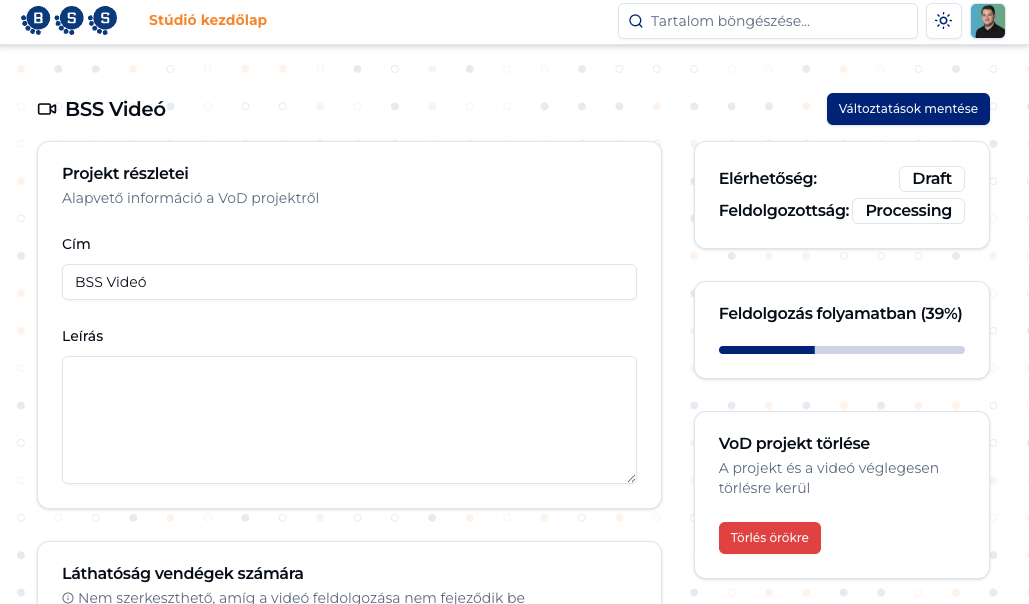
\includegraphics[width=150mm, keepaspectratio]{figures/processing.png}
  \caption{Képernyőkép egy videóprojekt szerkesztői nézetében.}
  \label{fig:processing}
\end{figure}

\Az+\refstruc{fig:processing} bemutatja, miképp kerül visszajelzésre a felületen az, hogy hol áll a feldolgozottsága egy feltöltött videónak. A képernyőképen jelzett ``BSS Videó'' nevű projektbe egy 91 MB-os 1 perc 43 másodperc hosszú videófájl került feltöltésre. A feldolgozást megvizsgáltam a MediaConvert konzoljáról, a job 42 másodpercig tartott. A feltöltött videó további paraméterei ezek voltak:

\begin{itemize}
  \setlength{\itemsep}{1pt}
  \setlength{\parskip}{0pt}
  \setlength{\parsep}{0pt}
  \item \textbf{Mozgóképanyag}: H.264 kódolású, 1920x1080p felbontás, 7 Mbps átlagos bitráta
  \item \textbf{Hanganyag}: AAC kódolás, 256 kbps bitráta, 2 csatorna, 48 kHz mintavételezés
\end{itemize}

\begin{figure}[h]
  \centering
  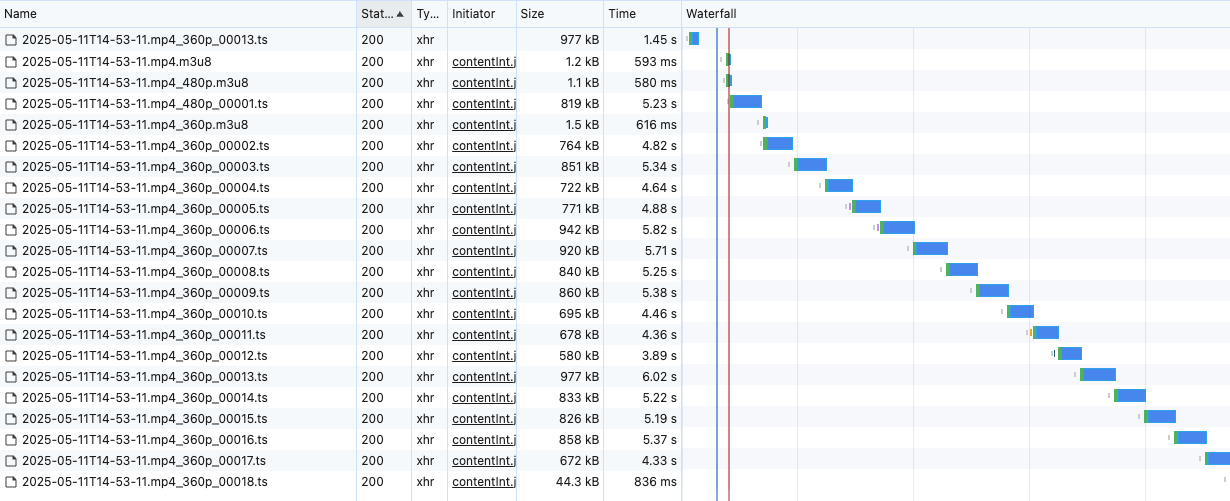
\includegraphics[width=150mm, keepaspectratio]{figures/browser_slow4g.png}
  \caption{Képernyőkép a HTTP-packetek érkezéséről (Slow 4G).}
  \label{fig:slow4g}
\end{figure}

\Az+\refstruc{fig:slow4g} mutatja be, ha átnavigálunk a weboldalon a streamelhető videó oldalára, akkor a böngészőben milyen packetek kerültek letöltésre a videófolyamokból. A böngészőben beállítottam sávszélkorlátozást (\emph{Slow 4G}), és azt tapasztaltam, hogy a böngésző elkezdi a 480p-s folyamot letölteni, majd az első packet után 360p-sre vált. A videót az~első packet megérkezése után rögtön elindítottam, a 360p-s videófolyam bufferelés nélkül tudott lejátszódni.

Kipróbáltam 3G-s beállítást is a Chrome böngészőben, azon a sávszélen már erősen hosszú bufferelésre volt szükség még a legalacsonyabb 360p-s felbontásnál is. Vártam másfél percet, hogy betöltsön néhány packetet előre a böngésző, utána már simább volt az élmény. Ez jelentős élményromlást tud jelenteni, ha egy körülbelül 2 perces videó lejátszásához is muszáj megállnom és bevárni pár packetet. Igény merülhet fel újabb és spórolósabb kimenetek bevezetésére a konvertálás folyamatába.
A 360p-s packetek átlagban 1,2 MB-osak lettek, a CDN a legtöbbet átlagban 800 kB-osra tudta letömöríteni még. Az 1080p-s packetek átlagban 10 MB-osak lettek, a 720p-sek 6 MB-osak, a 480p-sek 2,4 MB-osak. Ezek esetében is a CDN 30-40\% körüli tömörítést tudott elérni.

\subsection{A MediaConvert-job státuszváltozásának kezelése}

\Az+\ref{lst:emcEventRule}. kódrészlet mutatja be a MediaConvertben futó job eseményeire való feliratkozást. A~\verb|job-finalizer| modulbeli Lambda-függvény roppant egyszerű kóddal rendelkezik, csupán behív az eseményből kapott paraméterekkel (job ID és feldolgozottság százaléka) az~ALB-n keresztül a Node.js-appba a \verb|/api/videos/:id/progress| végponton, a webszerver pedig frissíti az adatbázisban a videó állapotát.

\begin{minipage}{0.92\textwidth}
  \begin{lstlisting}[
    caption=A streamzen-mediaconvert-event-rule-dev Terraform-kódja.,
    label=lst:emcEventRule,
    style=tf,
    basicstyle=\fontsize{10}{12}\ttfamily
  ]
resource "aws_cloudwatch_event_rule" "this" {
  name        = "streamzen-mediaconvert-event-rule-${var.environment}"
  description = "Capture MediaConvert job state changes"
  event_pattern = jsonencode({
    source      = ["aws.mediaconvert"],
    detail-type = ["MediaConvert Job State Change"]
    detail      = {
      status = ["COMPLETE", "ERROR", "STATUS_UPDATE"]
      userMetadata = {
        application = ["streamzen-${var.environment}"]
      }
    }
  })
}

resource "aws_cloudwatch_event_target" "this" {
  rule      = aws_cloudwatch_event_rule.this.name
  target_id = "streamzen-mediaconvert-event-target-${var.environment}"
  arn       = module.job_finalizer.arn
}
\end{lstlisting}
\end{minipage}

\section{A MediaLive és MediaPackage összekötése}\label{sec:mediaLive}

A MediaLive szolgáltatásban fellőttem a tervezett egyetlen csatornát, amelyre egy RTMP push alapú inputot kötöttem be. A létrehozott inputhoz az AWS rendelt IP-t, portot, a~kapott URL így ez lett: \url{rtmp://3.73.170.41:1935/streamzen-dev}. A csatorna úgy lett felkonfigurálva, hogy maximum 20 Mbps bitráta mellett 1080p-s felbontású videófolyamot tudjon fogadni, a hangot pedig AAC kódolásúként, 256 kbps bitrátával. A~MediaLive`|csatornából átvezetett folyam két kimenetet képez, egy 8 Mbps célbitrátájú 1080p-s kimenetet ad, illetve egy 3,3 Mbps célbitrátájú 720p-s kimenetet. A MediaPackage szolgáltatásban is egyetlen csatornát hoztam létre, amely a MediaLive-csatorna kimeneteit fogadja be, és az átkonvertálja HLS-formátumú folyamra.

A MediaLive-csatornának még szüksége volt egy IAM-szerepkörre, amelyben megadtam a szerepkörnek minden olyan jogosultságot, amely szükséges a MediaPackage`|csatornába való átvezetéshez számára, illetve a CloudWatch-ba való naplózásra és a szükséges hálózati/EC2-hez kapcsolódó jogokat is megkapta (a MediaLive hátterében menedzselt EC2-példányok futnak).

A MediaLive-csatorna indítása után lehetséges az input URL-re felcsatlakozva kezdeni a streamelést. Az RTMP streameléshez az OBS Studio nevű alkalmazást használtam\cite{obsMediaLive}, abban a beállításoknál a ``Stream'' menüben kitöltöttem az egyedi RTMP-szerverem adataival a mezőket (lásd \refstruc{fig:obs}). Nem került felhasználásra egyelőre a kísérlet alatt autentikáció a végpontra.

\begin{figure}[ht]
  \centering
  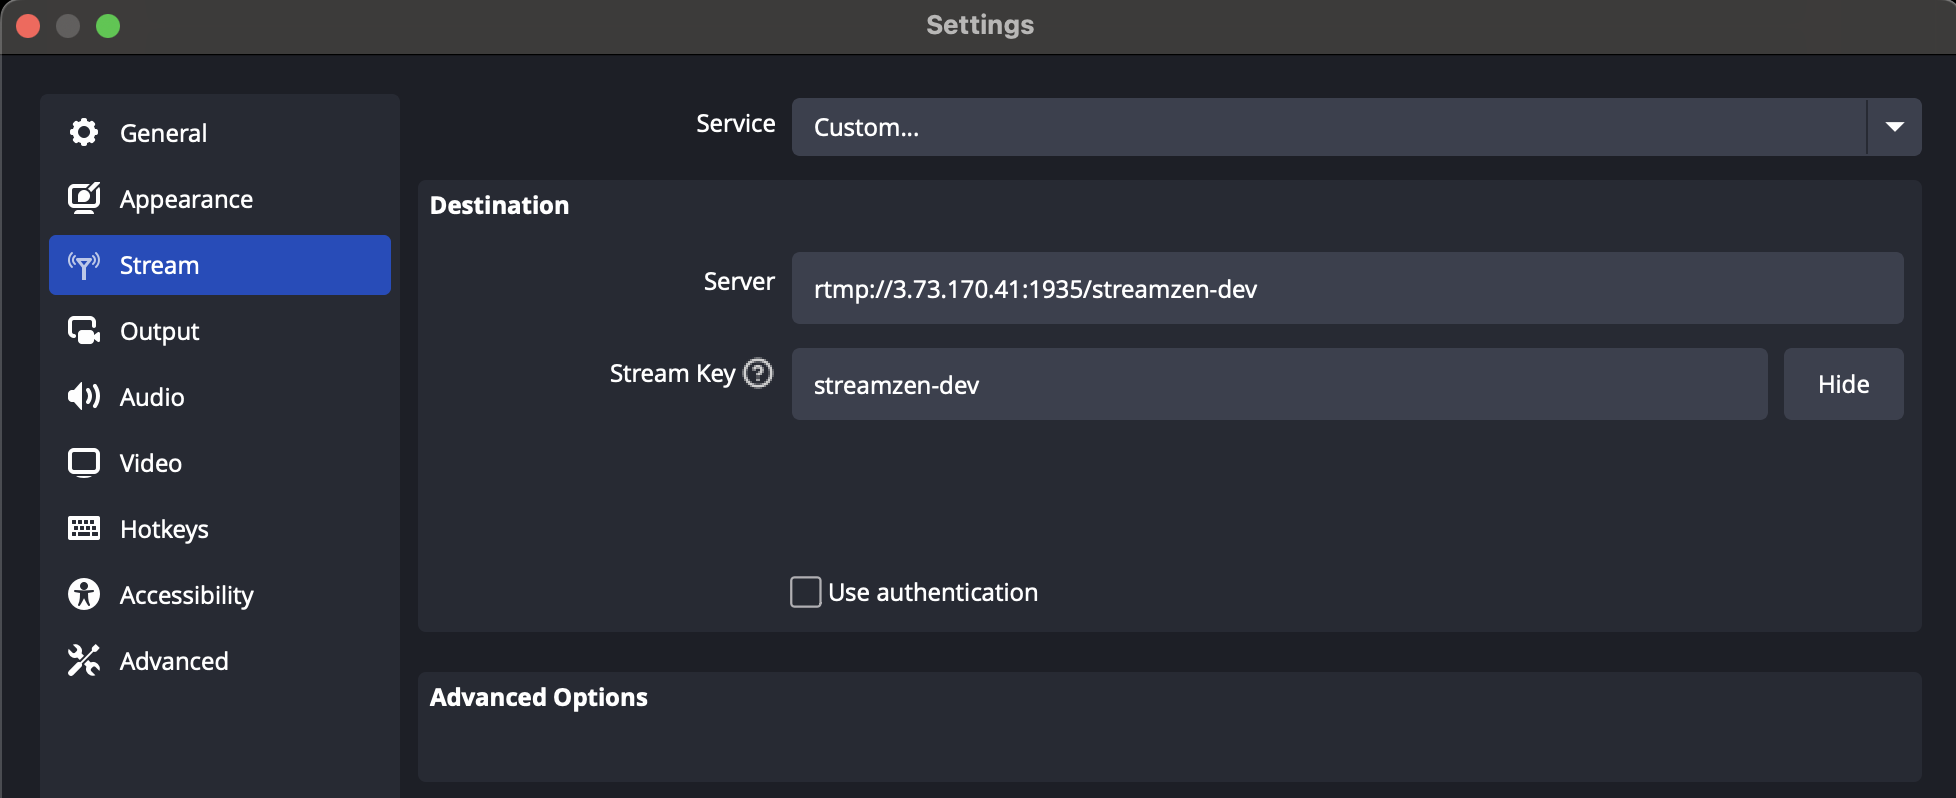
\includegraphics[width=150mm, keepaspectratio]{figures/obs.png}
  \caption{Képernyőkép az OBS stream beállításairól.}
  \label{fig:obs}
\end{figure}
